\chapter{Experiment}
\todo{ne tolle Einleitung schreiben}

\section{Setup A: Estimation of the quadrature point of the MZI modulator}
To calculate the quadrature point of the used MZI modulator the setup shown in figure \ref{fig:A_setup}\footnote[3]{Luca Alloatti, Materials for the preparation of OKT lab 8} was used. A laser source with an output wavelength of 1550~nm and an output power of 0~dBm were connected to an MZI modulator. The output of the MZI modulator was connected to a power meter. The modulator was biased over a variable DC voltage.

The DC voltage was swept from -4.8~V to 5.1~V in steps of 0.3~V. At every point the output power of the MZM was measured.

\begin{figure}%
\centering
\includegraphics[width=.5\columnwidth]{Grafiken/SetupA.png}%
\caption{Setup A}%
\label{fig:A_setup}%
\end{figure}

\begin{figure}%
\centering
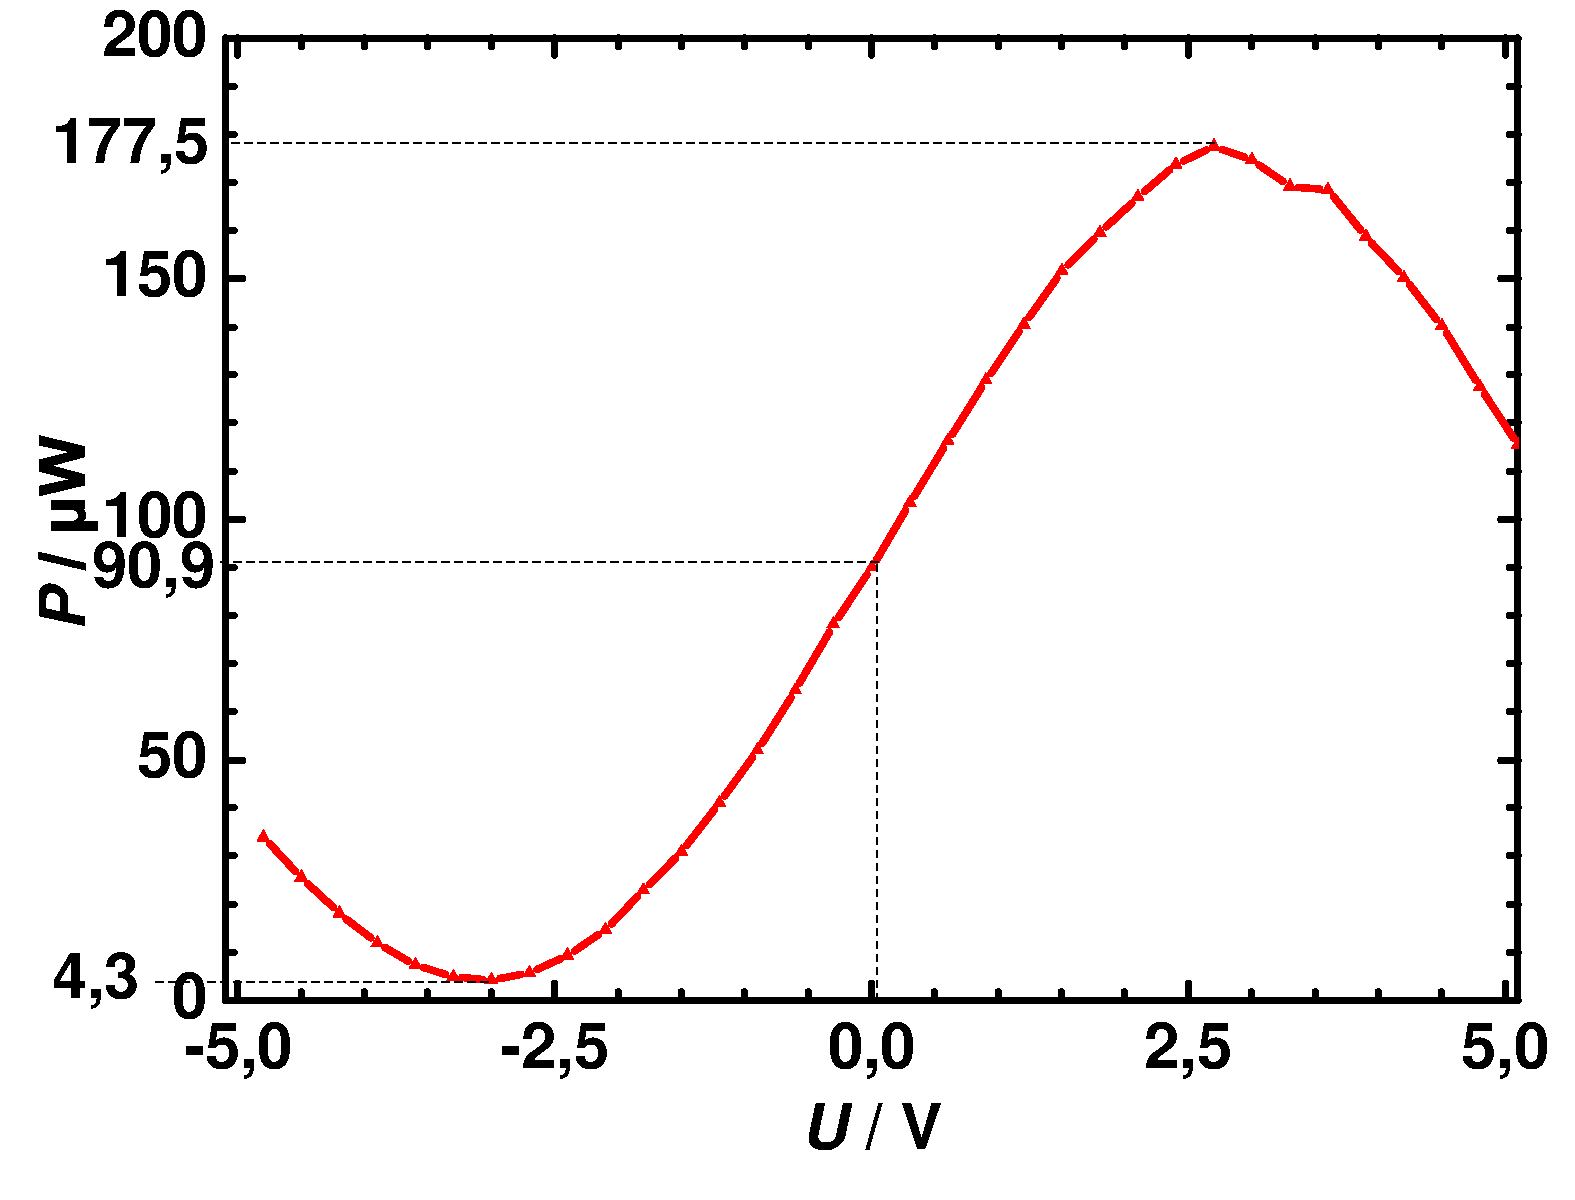
\includegraphics[width=.6\columnwidth]{Grafiken/A_quadratur.pdf}%
\caption{}%
\label{fig:A_quadratur}%
\end{figure}

Figure \ref{fig:A_quadratur} shows the recorded $P$/$U$ curve. It shows a good accordance to the squared sine $P$/$U$ curve of a theoretical MZI modulator.
The maximum optical output power of the MZI is at 2.5~V with 177.5~$\upmu$W. The minimal optical output power is at -3.0~V with 4.3~$\upmu$W. With this the quadrature point can be calculated to be at

\begin{equation}
P\i{out,quadrature}=\frac{177.5~\upmu \mathrm{W}+4.3~\upmu \mathrm{W}}{2}=90.9~\upmu \mathrm{W}\qquad.
\label{eq:}
\end{equation} 
Using a linear approximation in the quadrature point the corresponding voltage can be calculated.

\begin{equation}
\begin{split}
P\i{out}=90~\upmu \mathrm{W} + \frac{103.4~\upmu \mathrm{W}- 78.1~\upmu \mathrm{W}}{0.6~\mathrm{V}}\cdot U\\
U\i{quadrature}=\frac{90.9~\upmu \mathrm{W}-90~\upmu \mathrm{W}}{42.17~\upmu \mathrm{W}/\mathrm{V}}\\
=0.02~\mathrm{V} \quad.
\end{split}
\label{eq:}
\end{equation}
The quadrature point of the transfer function of the modulator was determined to be at $U\i{quadrature}\approx 0~\mathrm{V}$.


\section{Setup B: Optimization of the extinction ratio of the modulator; Q-factor measurement}





In the next Setup a bit pattern was modulated on the carrier and measured by a oscilloscope (Agilent 86100 Digital Communication Analyzer). To do so a pulse pattern generator was connected to the electrical input of the MZI modulator. The oscilloscope was connected to the output of the MZI modulator and to the electrical data output of the pulse pattern generator for optimal triggering. This setup is shown in figure \ref{fig:B_setup}\footnote[3]{Luca Alloatti, Materials for the preparation of OKT lab 8}.

Now the pulse pattern generator was set to the pseudo random bit sequence mode (PBRS) for transmitting patterns of the length PN23. The amplitudes of the electrical pulse and the clock were set to 1.0~V and 1.5~V without any offset, respectively.

\begin{figure}%
\centering
\includegraphics[width=.6\columnwidth]{Grafiken/B_setup.png}%
\caption{Setup B}%
\label{fig:B_setup}%
\end{figure} 


\section{Setup C: Receiver sensitivity measurement}

The MZM was connected to a variable optical attenuator set to the lowest possible attenuation. Then the output power was measured using the connected power meter. Figure \ref{fig:C_setup1}\footnote[3]{Luca Alloatti, Materials for the preparation of OKT lab 8} shows the used setup. For a laser output power of 0~dBm the output power was measured to be 63.5~$\upmu$W.

In the next step the power meter was disconnected and the photo receiver connected like shown in figure \ref{fig:C_setup2}\footnotemark[3]. The $DATA$ and the $CLOCK$ electrical outputs of the photo reciever were connected to the corresponding inputs of the BER analyzer. At the pulse pattern generator PRBS was set as the data signal. The BER analyzer was set to $AUTOSEARCH$ in the $TIMED$ test mode. 
\begin{figure}%
\centering
\includegraphics[width=.6\columnwidth]{Grafiken/C_setup1.png}%
\caption{Setup C.1}%
\label{fig:C_setup1}%
\end{figure}



\begin{figure}%
\centering
\includegraphics[width=.6\columnwidth]{Grafiken/C_setup2.png}%
\caption{Setup C.2}%
\label{fig:C_setup2}%
\end{figure}



\begin{figure}%
\centering
\includegraphics[width=.6\columnwidth]{Grafiken/BER.pdf}%
\caption{BER for different bit patterns.}%
\label{fig:BER}%
\end{figure}
\todo{hier fehlt noch warums mit 1mW net richtig geklappt hat}
The output power of the laser was now set to 3~mW. With the variable optical attenuatior the power at the photo diode was varied and the BER was measured. Figure \ref{fig:BER} shows the dependence of the BER on the optical power for a bit squences of the length \textit{PN~17} and \textit{PN~20}, respectively. In the \textit{PN~17} bit sequence one can see, that the BER decreases with increasing power. This can be explained by the fact that the signal in the optical transmission system is a poisson process. When the power is doubled the noise only increases by a factor of $\sqrt{2}$. 
\todo{PN20, ich wei� nimmer warum die BER auch vom Bitpattern abh�ngt.}



\todo{Damit du die daten hast: Nach erneutem Einstellen und 3~mW laserleistung: gemesseN. -4.3~dBm bzw. 0.3824~mW}